\section{EXPERIMENTS}
In this section, we show the efficacy of the proposed methods using toy Gaussian models and the MNIST dataset.
\subsection{Projection Method}
To prove the effectiveness of our projection method compared with the traditional projection method in the Lasso problem, we compared the projection distance and screening ratio with randomly generated Gaussian measures by two projection methods. We set the $\lambda = \frac{\|\mathbf{X}^{\tranT}y\|}{100}$ and test for 10 different pairs.We choose the FISTA for solving the $L_2$ penalized UOT problems. Our projection method has only moved the dual point by a very small order of magnitude. It ensures that the points are kept at a smaller distance from the optimal solution and cause better screening effects.
	\begin{figure}[h]
	\begin{center}	
	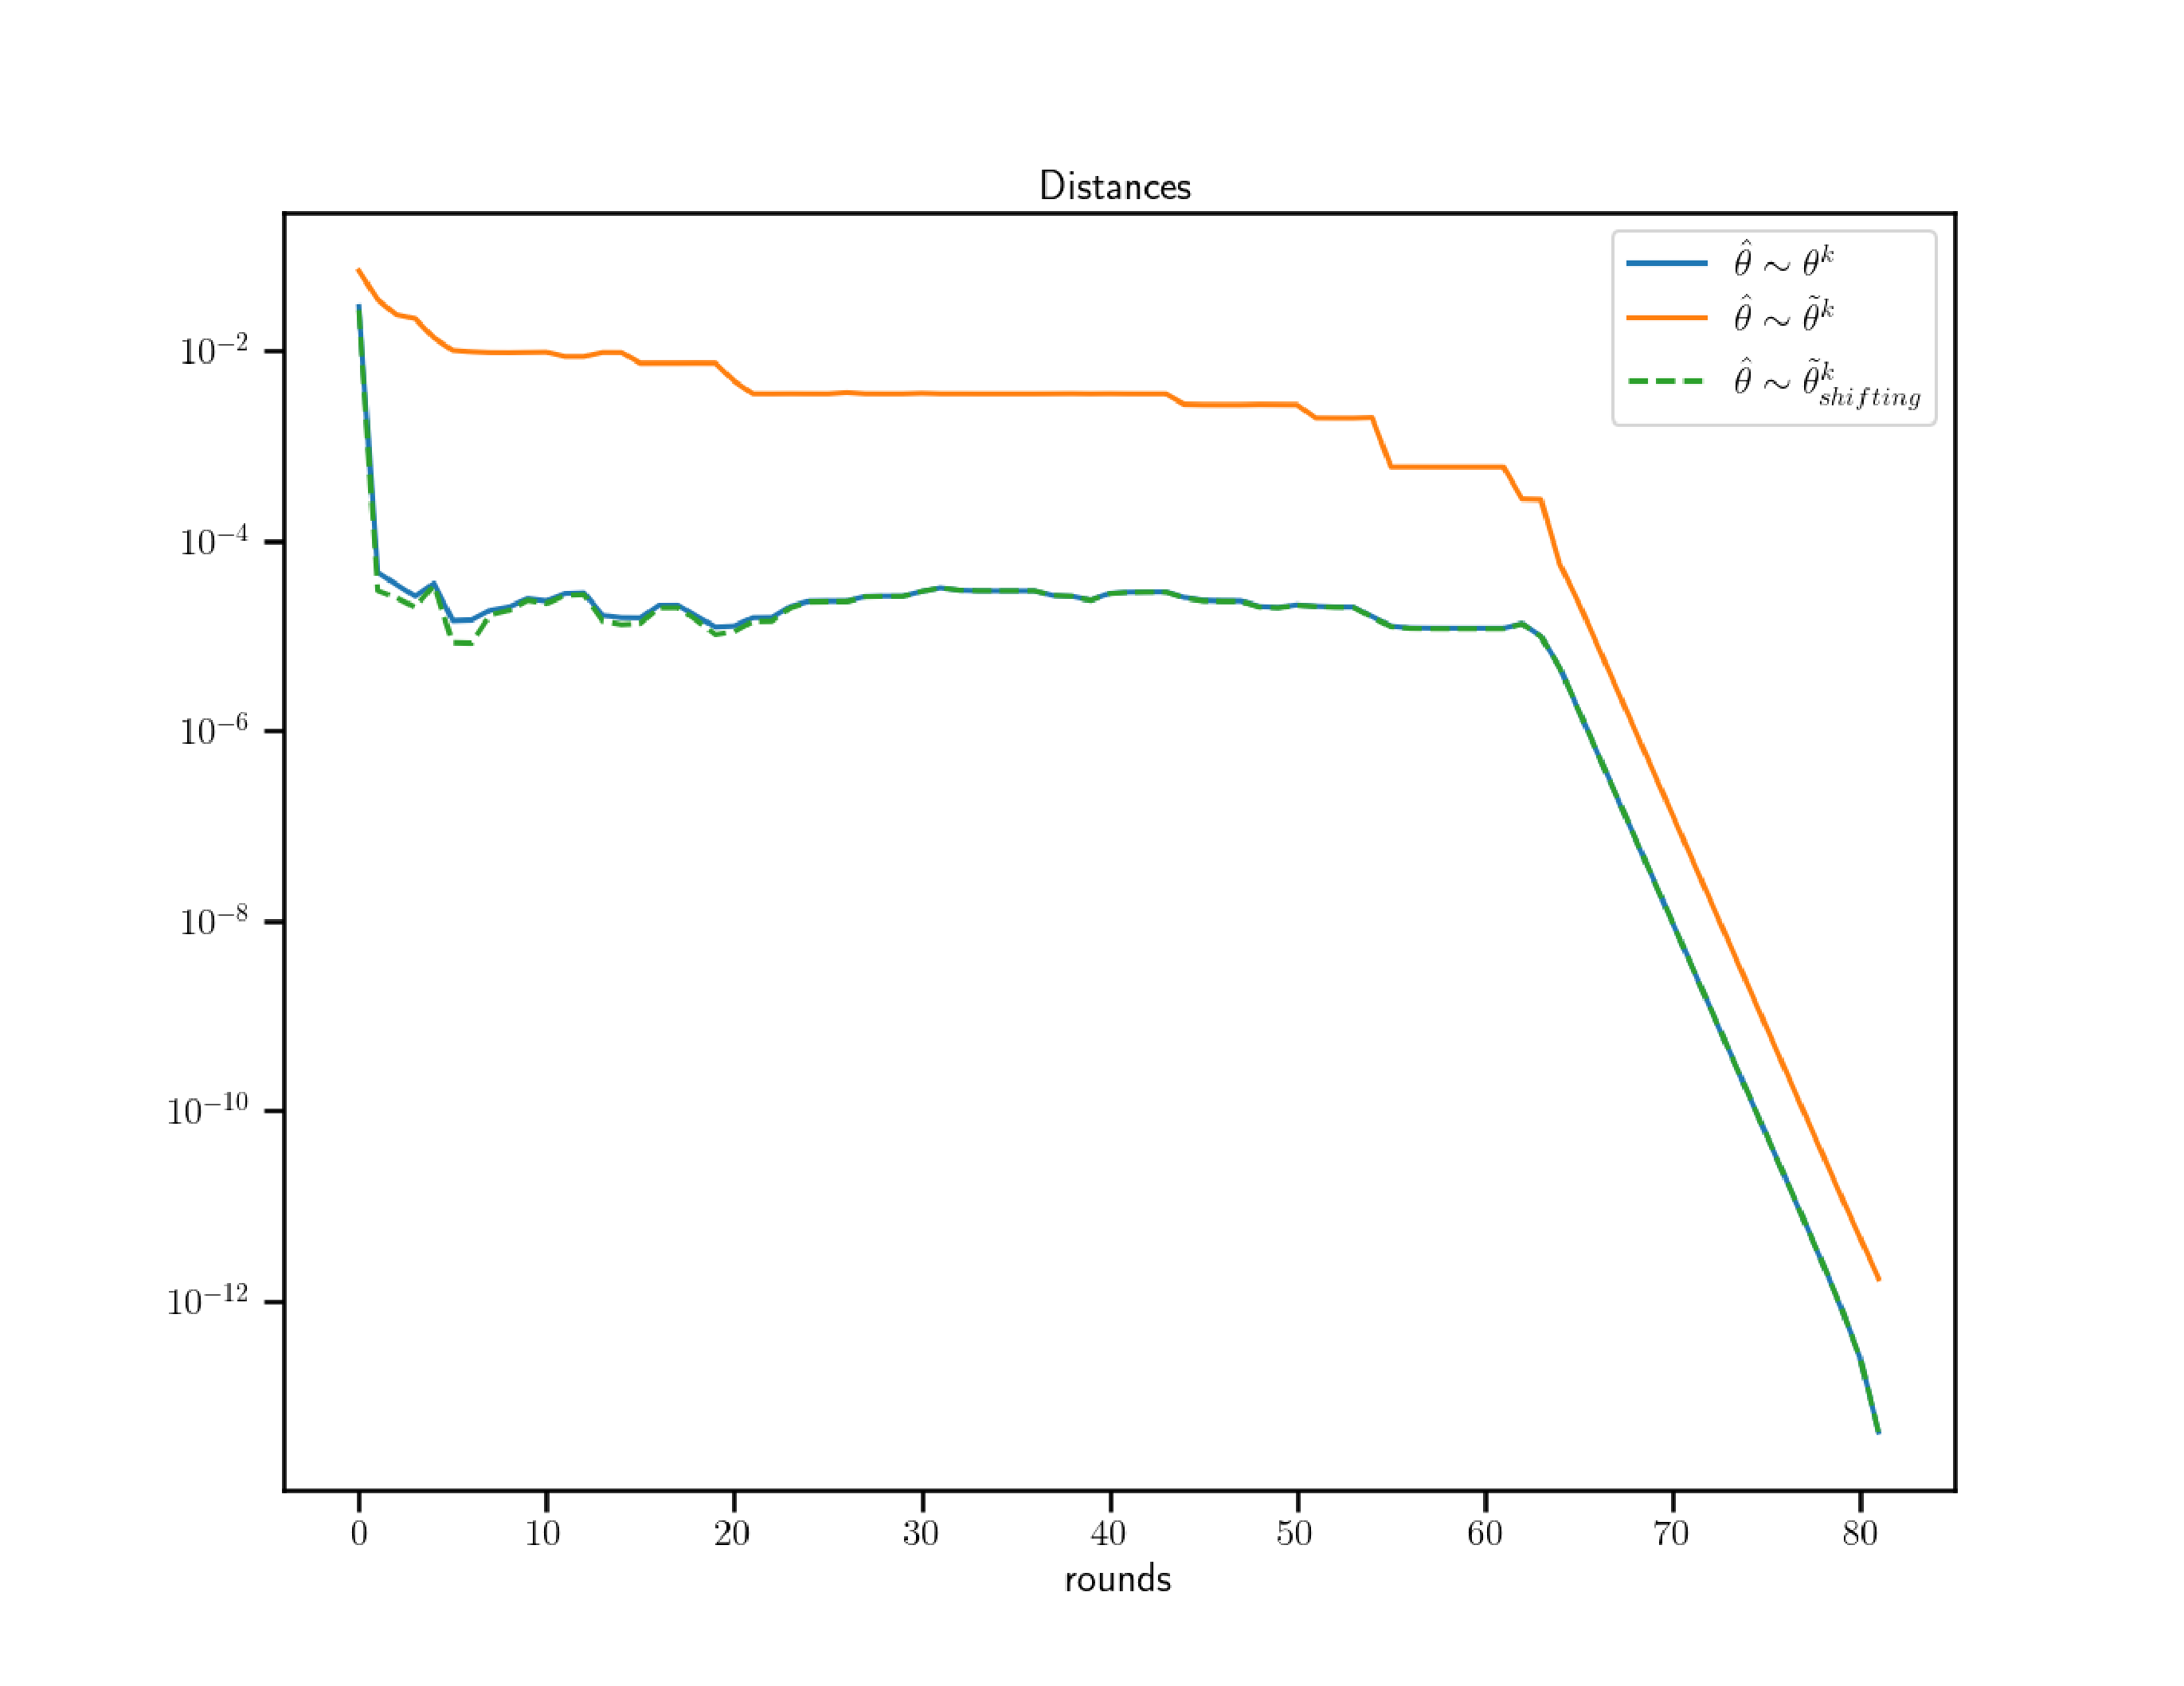
\includegraphics[width = \linewidth]{pic/projdis}
	\caption{Distance of different projection method}
	\end{center}	
	\end{figure}
	\begin{figure}[htbp]
	\begin{center}	
	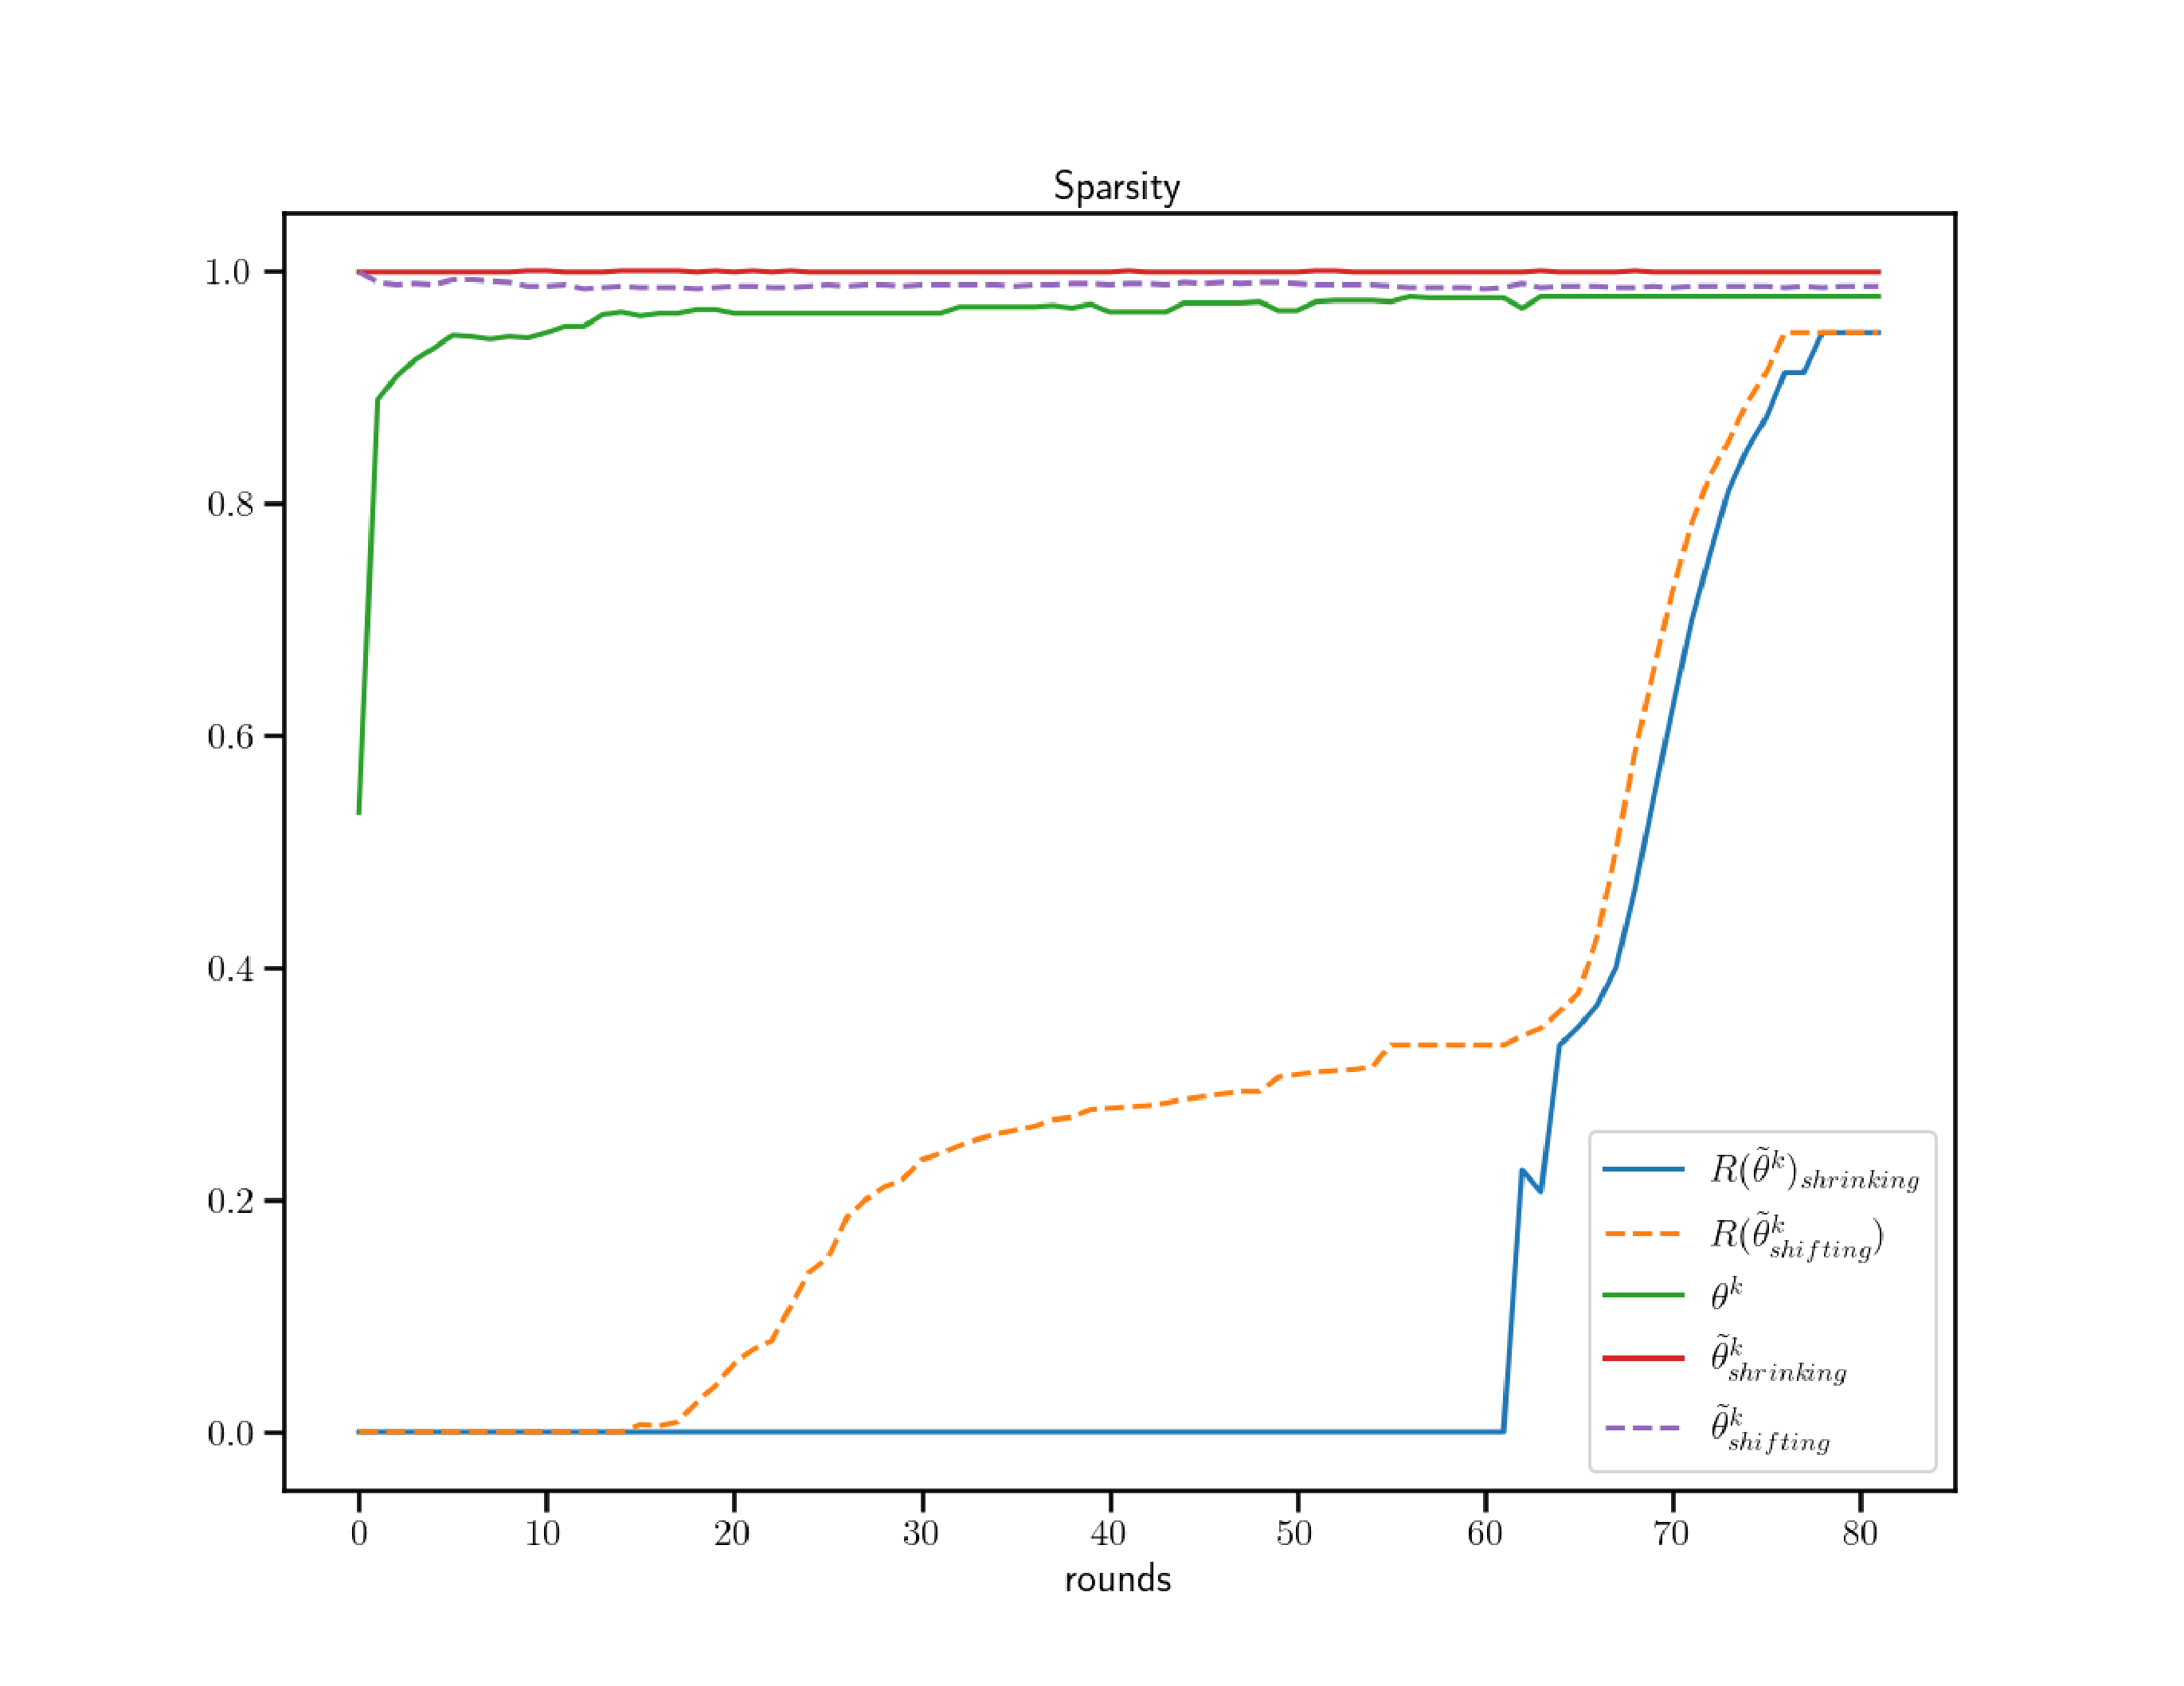
\includegraphics[width = \linewidth]{pic/sparse_proj}
	\caption{Screening ratio of different projection method}
	\end{center}	
	\end{figure}

\subsection{Divide Method}
We compared the screening ratio with three different methods, including our Divide method, Dynamic Sasvi method, and Gap method. Every method would use our projection method to get a better outcome, which also makes sure the difference in performance is only in the construction of the feasible domain. 
	\begin{figure}[h]
	\begin{center}	
	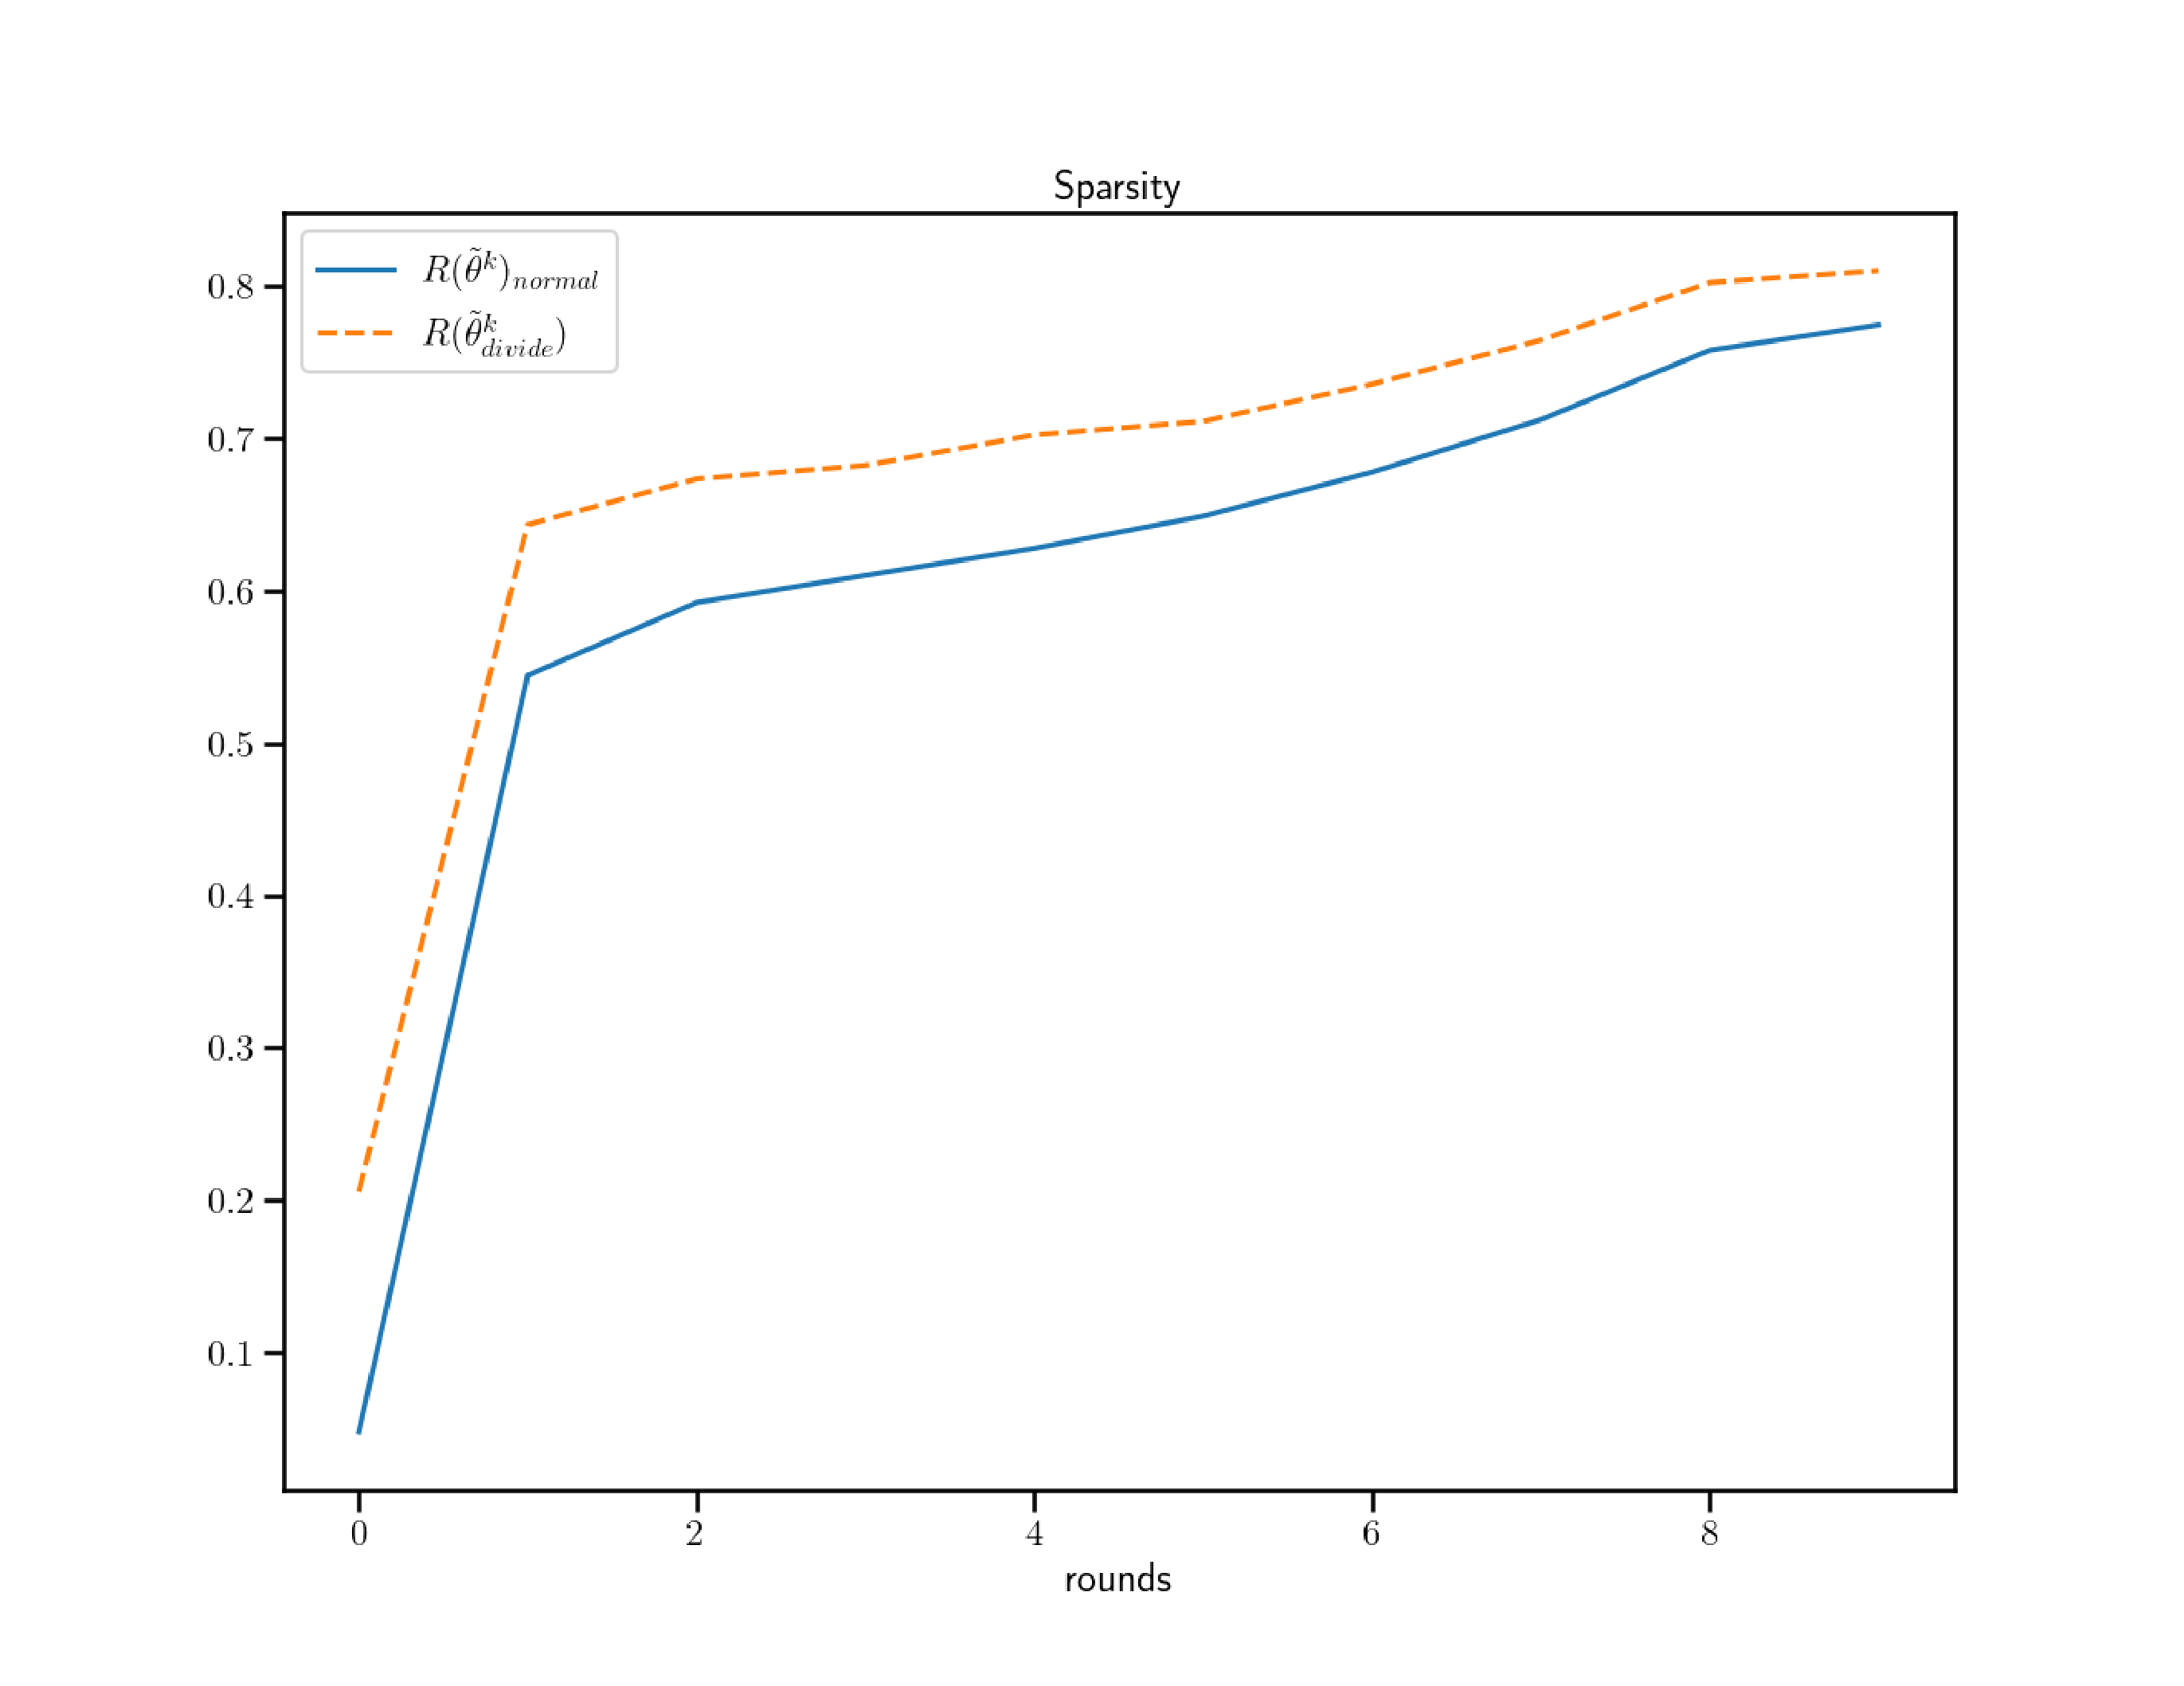
\includegraphics[width = \linewidth]{pic/screening_divide_ratio_long}
	\caption{Screening ratio of dividing method}
	\end{center}	
	\end{figure}

\subsection{Best Divide Method}
We compared the screening ratio with three different methods, including our Divide method, the Dynamic Sasvi method, and a random divide method. 
	\begin{figure}[h]
	\begin{center}	
	\includegraphics[width = \linewidth]{pic/divide}
	\caption{Comparing of our separation method with random separation method}
	\end{center}	
	\end{figure}

\subsection{Speed up Ratio}

We choose the FISTA method, Newton method, and Language method to test the screening ratio. 
	\begin{figure}[h]
	\begin{center}	
	\includegraphics[width = \linewidth]{pic/divide}
	\caption{speed up ratio for different solver}
	\end{center}	
	\end{figure}